%!TEX program = xelatex

\documentclass[11pt,titlepage]{report}
%!TEX root = main.tex

\usepackage[T1]{fontenc}
\usepackage{lmodern}
\usepackage[svgnames]{xcolor}
\usepackage{fontspec} % XeLaTeX required!
\usepackage{graphicx}
\usepackage{circuitikz}
\usepackage{tikz}
\usepackage{pifont}
\usepackage[some]{background}
\usepackage{xltxtra} 
\usepackage{setspace}
\usepackage[absolute]{textpos}
\usepackage[latin1]{inputenc}
\usepackage[english]{babel}
\usepackage{graphicx}
\usepackage{wrapfig}
\usepackage{fullpage}
\usepackage[margin=1in]{geometry}
\usepackage{float}
\usepackage{url}
\usepackage{multicol}
\usepackage{hyperref}
\usepackage{titlepic}
\usepackage{standalone}
\usepackage{siunitx}
\usepackage{booktabs}
\usepackage{amsmath}
\usepackage{unicode-math}
\usepackage{verbatim}
\usepackage{enumitem}
\usepackage{listings}
\usepackage{multirow}
\usepackage{pgfplots}
\pgfplotsset{compat=1.8}
\usepackage{caption} 
\usepackage[parfill]{parskip}
\usepackage{import}
\usepackage[backend=bibtexu,texencoding=utf8,bibencoding=utf8,style=ieee,sortlocale=en_GB,language=auto]{biblatex}
\usepackage[strict,autostyle]{csquotes}
\usepackage[final]{pdfpages}
\usepackage{subcaption}
\usepackage{ifplatform}
%\captionsetup[table]{skip=10pt}


% Fix for includepdf bug in Mac OS X
\newcommand{\insertpdfpath}[1]{
	\ifwindows
	\newcommand{\insertpdf}[2]{\includepdf[pages=##1]{##2}}
	\else
	\newcommand{\insertpdf}[2]{\includepdf[pages=##1]{#1/##2}}
	\fi
}

%set fonts
\setmainfont[Ligatures=TeX]{Myriad Pro}
\setmathfont{Asana Math}
\setmonofont{Lucida Console}

\usepackage{titlesec, color}
\renewcommand{\familydefault}{\sfdefault} %set font family
\renewcommand{\arraystretch}{1.2} %set table vertical spacing
\setlength\parindent{0pt} %no paragraph indent
\hypersetup{ %setup hyperlinks
    colorlinks,
    citecolor=black,
    filecolor=black,
    linkcolor=black,
    urlcolor=black
}

%redesign chapter headings
\definecolor{gray75}{gray}{0.75}
\newcommand{\chapternumber}{\thechapter}
\newcommand{\hsp}{\hspace{20pt}}
\titleformat{\chapter}[hang]{\Huge\bfseries}{\chapternumber\hsp\textcolor{gray75}{|}\hsp}{0pt}{\Huge\bfseries}

%Redefine appendix headers
\renewcommand{\appendixname}{Appendix}
\renewcommand{\appendixtocname}{Appendices}
\renewcommand{\appendixpagename}{Appendices}

%For code listings
\definecolor{black}{rgb}{0,0,0}
\definecolor{browntags}{rgb}{0.65,0.1,0.1}
\definecolor{bluestrings}{rgb}{0,0,1}
\definecolor{graycomments}{rgb}{0.4,0.4,0.4}
\definecolor{redkeywords}{rgb}{1,0,0}
\definecolor{bluekeywords}{rgb}{0.13,0.13,0.8}
\definecolor{greencomments}{rgb}{0,0.5,0}
\definecolor{redstrings}{rgb}{0.9,0,0}
\definecolor{purpleidentifiers}{rgb}{0.01,0,0.01}


\lstdefinestyle{csharp}{
language=[Sharp]C,
showspaces=false,
showtabs=false,
breaklines=true,
showstringspaces=false,
breakatwhitespace=true,
escapeinside={(*@}{@*)},
columns=fullflexible,
commentstyle=\color{greencomments},
keywordstyle=\color{bluekeywords}\bfseries,
stringstyle=\color{redstrings},
identifierstyle=\color{purpleidentifiers},
basicstyle=\ttfamily\small}

\lstdefinestyle{c}{
language=C,
showspaces=false,
showtabs=false,
breaklines=true,
showstringspaces=false,
breakatwhitespace=true,
escapeinside={(*@}{@*)},
columns=fullflexible,
commentstyle=\color{greencomments},
keywordstyle=\color{bluekeywords}\bfseries,
stringstyle=\color{redstrings},
identifierstyle=\color{purpleidentifiers},
}

\lstdefinestyle{matlab}{
language=Matlab,
showspaces=false,
showtabs=false,
breaklines=true,
showstringspaces=false,
breakatwhitespace=true,
escapeinside={(*@}{@*)},
columns=fullflexible,
commentstyle=\color{greencomments},
keywordstyle=\color{bluekeywords}\bfseries,
stringstyle=\color{redstrings},
identifierstyle=\color{purpleidentifiers}
}

\lstdefinestyle{vhdl}{
language=VHDL,
showspaces=false,
showtabs=false,
breaklines=true,
showstringspaces=false,
breakatwhitespace=true,
escapeinside={(*@}{@*)},
columns=fullflexible,
commentstyle=\color{greencomments},
keywordstyle=\color{bluekeywords}\bfseries,
stringstyle=\color{redstrings},
identifierstyle=\color{purpleidentifiers}
}

\lstdefinestyle{xaml}{
language=XML,
showspaces=false,
showtabs=false,
breaklines=true,
showstringspaces=false,
breakatwhitespace=true,
escapeinside={(*@}{@*)},
columns=fullflexible,
commentstyle=\color{greencomments},
keywordstyle=\color{redkeywords},
stringstyle=\color{bluestrings},
tagstyle=\color{browntags},
morestring=[b]",
  morecomment=[s]{<?}{?>},
  morekeywords={xmlns,version,typex:AsyncRecords,x:Arguments,x:Boolean,x:Byte,x:Char,x:Class,x:ClassAttributes,x:ClassModifier,x:Code,x:ConnectionId,x:Decimal,x:Double,x:FactoryMethod,x:FieldModifier,x:Int16,x:Int32,x:Int64,x:Key,x:Members,x:Name,x:Object,x:Property,x:Shared,x:Single,x:String,x:Subclass,x:SynchronousMode,x:TimeSpan,x:TypeArguments,x:Uid,x:Uri,x:XData,Grid.Column,Grid.ColumnSpan,Click,ClipToBounds,Content,DropDownOpened,FontSize,Foreground,Header,Height,HorizontalAlignment,HorizontalContentAlignment,IsCancel,IsDefault,IsEnabled,IsSelected,Margin,MinHeight,MinWidth,Padding,SnapsToDevicePixels,Target,TextWrapping,Title,VerticalAlignment,VerticalContentAlignment,Width,WindowStartupLocation,Binding,Mode,OneWay,xmlns:x}
}

\lstdefinestyle{matlab}{
language=Matlab,
showspaces=false,
showtabs=false,
breaklines=true,
showstringspaces=false,
breakatwhitespace=true,
escapeinside={(*@}{@*)},
columns=fullflexible,
commentstyle=\color{greencomments},
keywordstyle=\color{bluekeywords}\bfseries,
stringstyle=\color{purpleidentifiers},
identifierstyle=\color{purpleidentifiers}
}

%defaults
\lstset{
basicstyle=\ttfamily\small,
extendedchars=false,
numbers=left,
numberstyle=\ttfamily\tiny,
stepnumber=1,
tabsize=4,
numbersep=5pt
}
\addbibresource{../../library/bibliography.bib}

\begin{document}

\chapter{Assignment 1}
\section{Task 1}

Following the definition for the characteristic impedance $Z_0$ and substituting $Z_s=\frac{1}{j\omega C}$ and $Z_p=j\omega L$ gives:

\begin{align}
	Z_0 &=\frac{Z_s}{2} + \sqrt{\frac{Z_s^2}{4}+Z_sZ_p} \nonumber \\
	&= \frac{1}{2j\omega C} + \sqrt{\frac{L}{C}-\frac{1}{4\omega^2C^2}} 
\end{align}

For the propagation coefficient we have that $\gamma = 1-\frac{Z_s}{Z_0}$, in which $Z_s$ and $Z_0$ may be substituted and the result simplified:

\begin{align}
	\gamma &= 1 - \frac{1}{ j\omega C\left( \frac{1}{2\omega C} + \sqrt{\frac{L}{C}-\frac{1}{4\omega^2C^2}}\right)}
	\\
	&= 1 - \frac{1}{\frac{1}{2}+\sqrt{\frac{1}{4}-LC\omega^2}} = \frac{-\frac{1}{2}+\sqrt{\frac{1}{4}-LC\omega^2}}{\frac{1}{2}+\sqrt{\frac{1}{4}-LC\omega^2}}
\end{align}

From this last equality, the frequency behavior of the ladder network may be obtained.
\\
If $\omega\geq\sqrt{\frac{1}{4LC}}$, $\sqrt{\frac{1}{4}-LC\omega^2}$ will equal an imaginary number which we shall call $jX$:

\begin{align}
	\lvert\gamma\rvert &= \frac{\lvert -\frac{1}{2}+jX \rvert}{\lvert \frac{1}{2}+jX \rvert} = 
	\frac{\sqrt{\frac{1}{4}+X^2}}{\sqrt{\frac{1}{4}+X^2}}=1.
\end{align}

If $\omega < \sqrt{\frac{1}{4LC}}$, $\sqrt{\frac{1}{4}-LC\omega^2}$ will equal a positive real number which we shall call $X$:

\begin{equation}
	\lvert\gamma\rvert = \frac{\lvert -\frac{1}{2}+X \rvert}{\lvert \frac{1}{2}+X \rvert}.
\end{equation}

Since $X$ is positive, $\lvert\gamma\rvert < 1$ for all $\omega < \sqrt{\frac{1}{4LC}}$. 

From this we may conclude that the ladder network is a high-pass network, because the transfer is unity for high frequencies and less than one for low frequencies. This was to be expected expected, since the ladder network described in section 5.1.2 of the student manual is a low-pass filter and in this scenario the inductor and capacitor have changed places, yielding the dual case: a high-pass filter \cite[60]{epo4-manual}. The crossover (or cutoff) frequency is the frequency on the border of unity gain and lower gain: $\omega_0=\sqrt{\frac{1}{4LC}}$.

\section{Task 2}
The general equation for the voltage across the channel is 

\begin{equation}
	V(z,t)=U(t-\gamma z) + \Gamma U(t+\gamma(z-2l))-\Gamma U(t-\gamma(z+2l))-\Gamma^2U(t+\gamma(z-4l))\dots
\end{equation}

in which $\Gamma=\frac{Z_l-Z_0}{Z_l+Z_0}$ as stated in the student manual \cite[64]{epo4-manual}.

For the case when $z=l$, with open-circuited terminals, $Z_l \to \infty$, so $\Gamma=1$ and thus:

\begin{equation}
	V(z,t)=U(t-\gamma z) + U(t+\gamma(z-2l))- U(t-\gamma(z+2l))- U(t+\gamma(z-4l))\dots
\end{equation}

For the case when $z=l$, with short-circuited terminals, $Z_l \to 0$, so $\Gamma=-1$ and thus:

\begin{equation}
	V(z,t)=U(t-\gamma z) - U(t+\gamma(z-2l))+U(t-\gamma(z+2l))-U(t+\gamma(z-4l))\dots
\end{equation}


\section{Task 3}
The characteristic impedance may be found using the formula $Z_0=\sqrt{\frac{L_0}{C_0}}$. For this particular case this gives $Z_0=\sqrt{\frac{0.5\cdot10^-6}{2\cdot10^-9}}= \SI{18.5}{\ohm}$.

\begin{figure}[H]
	\centering
	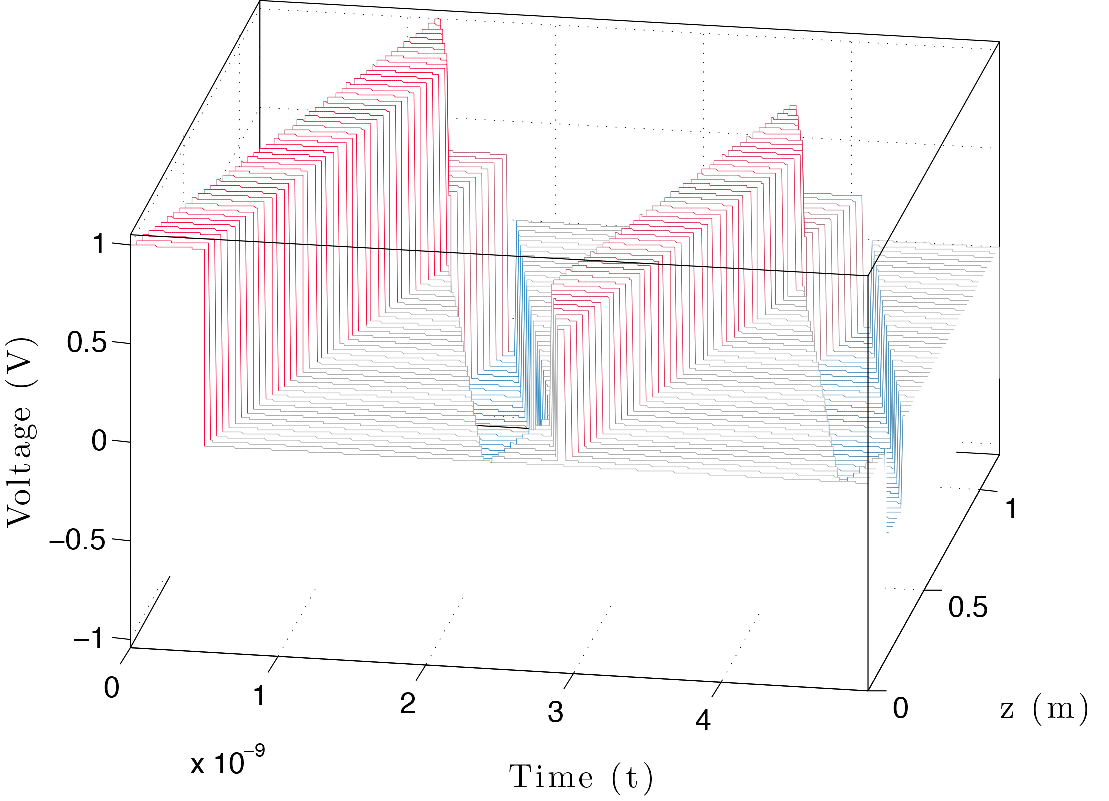
\includegraphics[width=.85\linewidth]{resource/voltage-cropped.pdf}
	\caption{Space-time plot of the voltage across the channel}
	\label{fig:ass1-voltage}
\end{figure}

The space-time plot of the voltage in the line is given in Figure~\ref{fig:ass1-voltage}. This plot was obtained using the given \texttt{MATLAB} function \texttt{bscan\_plot} along with the fact that $\Gamma=\frac{Z_l-Z_0}{Z_l+Z_0}$ and some \texttt{MATLAB} functions for calculating the voltage at $x=0$ at a given time and calculating $V(z,t)$ for a given $z,t$. Source code of every used \texttt{MATLAB}-file may be found in Appendix~\ref{appsec:task3}.

Interesting to note about the voltage is that it moves back and forth (reflects) throughout the transmission line: the voltage is positive on the way from $x=0$ to $x=\SI{1.2}{m}$ and negative on its way back. The voltage is $\SI{\pm1}{V}$ throughout the line, except at the load, where it is lower. However, because power is dissipated, the voltage does fade over time.

\begin{figure}[H]
	\centering
	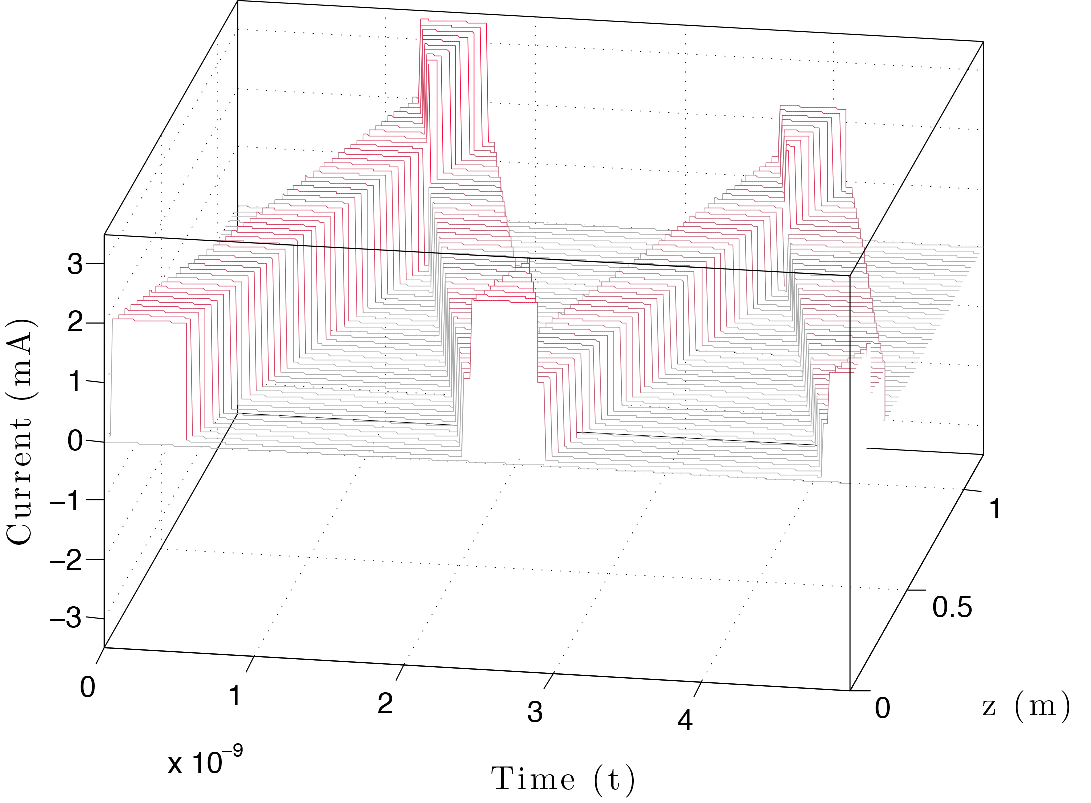
\includegraphics[width=.85\linewidth]{resource/current-cropped.pdf}
	\caption{Space-time plot of the current across the channel}
	\label{fig:ass1-current}
\end{figure}

The space-time plot of the current in the transmission line is given in Figure~\ref{fig:ass1-current}. Interestingly, there are two ways of calculating the current from equations (5.13) and (5.14) in the student manual, either by spatially integrating the voltage: (5.13) or by integrating the voltage with respect to time: (5.14) \cite[62]{epo4-manual}. We chose the former, in the following way:

\begin{align}
\frac{\partial I(z,t)}{\partial z} &= 
-C_0\frac{\partial V(z,t)}{\partial t} = I(z,t)=-C_0\int \! \frac{\partial V(z,t)}{\partial t}\, \mathrm{d}z \nonumber
\\
&\approx -C_0\sum\frac{V(z,t+\Delta t)-V(z,t)}{\Delta t}\Delta z
\end{align}

In this way, $I(z,t)$ can be approximated by numerically integrating the voltage. 

The current plot also has some interesting features: it also produces traveling waves back and forth through the line, although the current is positive at all times. It can also be seen that the initial condition, $I(0,0)=0$, holds: the current is zero at the origin of the wave. Moreover, the current does not instantaneously change after $t=0$, as expected. Just like the voltage, the current also fades over time.

\section{Task 4}
The general reflection coefficient is given by 

\begin{equation}
	\hat{\Gamma}(s)=\frac{Z_l-Z_0}{Z_l+Z_0},
\end{equation}

which in this case reduces to

\begin{equation}
	\Gamma = \frac{Z_l-Z_0}{Z_l+Z_0}=\frac{50+j50-15.8}{50+j50+15.8}=0.70+j0.23,
\end{equation}

because the latter is frequency independent.

Assuming the same feeding voltage pulse as in the previous exercise, we can Fourier transform the expression and use it to calculate $V(z,j\omega)$ using equation (5.29) from the student manual, along with the found $\Gamma$ and the fact that $\beta=\omega\gamma=\omega\sqrt{C_0L_0}$ \cite[63]{epo4-manual}. Because $U(t)=\epsilon(t)-\epsilon(t-t_w)$, it holds that $U(j\omega)=(\pi\delta(\omega)+\frac{1}{j\omega})(1-e^{-j\omega t_w})$.

Given the above, we can use \texttt{MATLAB} to create a Bode (magnitude) plot for $V(z,j\omega)\mid_{z=l=1.2}$. The code can be found in Appendix~\ref{appsec:task4}.
Interesting to note is that the bode plot represents a low pass filter with a $f_{-3dB}$ of around \SI{10}{\mega\hertz}. Then, around \SI{1}{\giga\hertz} some interesting phenomena occur. A more detailed plot of this region can be found in Figure~\ref{fig:ass1-esd}. We observe equally spaced peaks spaced about \SI{2.5}{\giga\hertz} apart.

\begin{figure}[H]
	\centering
	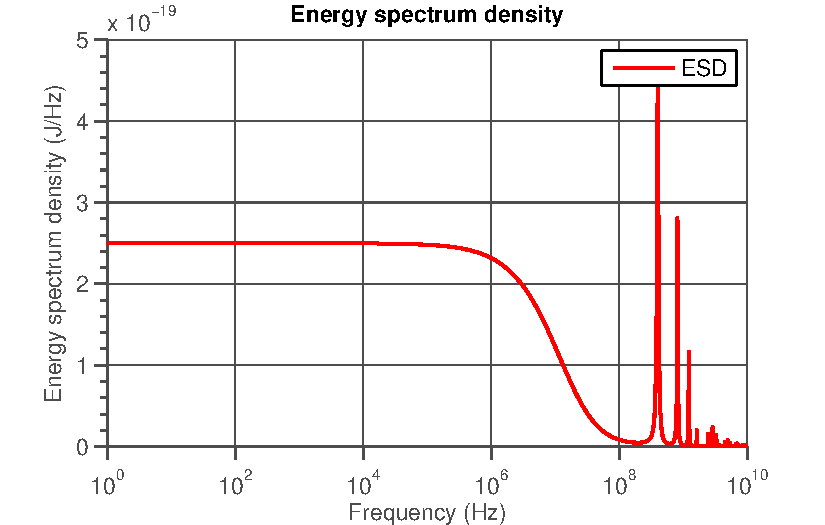
\includegraphics[width=.85\linewidth]{resource/esd.pdf}
	\caption{ESD of $y(t)$}
	\label{fig:ass1-esd}
\end{figure}

Because it is difficult to define the efficiency of power transfer in the case of complex loads with no frequency dependency, we decided to use the voltage transfer as a measure of power efficiency. Note that

\begin{align}
	\eta_{\text{power}}=\frac{P_{out}}{P_{in}} \times 100\% = 
	\frac{\frac{V_{out}^2}{Z_l}}{\frac{V_{in}^2}{Z_{in}}}*100\% =
	\eta_{\text{voltage}} \times \frac{Z_l}{Z_{in}}.
\end{align}

We conclude assignment 1 by calculating $\eta_{\text{voltage}}=\frac{V_{out}^2}{V_{in}^2}$, using \texttt{MATLAB} to integrate the voltage transfer function used to create the bode plot, resulting in $\eta_{\text{voltage}}\approx 20\%$.

\end{document}